%% Nothing to modify here.
%% make sure to include this before anything else

\documentclass[10pt]{beamer}
\usetheme{Szeged}

% packages
\usepackage{color}
\usepackage{listings}

% color definitions
\definecolor{mygreen}{rgb}{0,0.6,0}
\definecolor{mygray}{rgb}{0.5,0.5,0.5}
\definecolor{mymauve}{rgb}{0.58,0,0.82}

% re-format the title frame page
\makeatletter
\def\supertitle#1{\gdef\@supertitle{#1}}%
\setbeamertemplate{title page}
{
  \vbox{}
  \vfill
  \begin{centering}
  \begin{beamercolorbox}[sep=8pt,center]{title}
      \usebeamerfont{supertitle}\@supertitle
   \end{beamercolorbox}
    \begin{beamercolorbox}[sep=8pt,center]{title}
      \usebeamerfont{title}\inserttitle\par%
      \ifx\insertsubtitle\@empty%
      \else%
        \vskip0.25em%
        {\usebeamerfont{subtitle}\usebeamercolor[fg]{subtitle}\insertsubtitle\par}%
      \fi%     
    \end{beamercolorbox}%
    \vskip1em\par
    \begin{beamercolorbox}[sep=8pt,center]{author}
      \usebeamerfont{author}\insertauthor
    \end{beamercolorbox}
    \begin{beamercolorbox}[sep=8pt,center]{institute}
      \usebeamerfont{institute}\insertinstitute
    \end{beamercolorbox}
    \begin{beamercolorbox}[sep=8pt,center]{date}
      \usebeamerfont{date}\insertdate
    \end{beamercolorbox}\vskip0.5em
    {\usebeamercolor[fg]{titlegraphic}\inserttitlegraphic\par}
  \end{centering}
  \vfill
}
\makeatother

% insert frame number
\expandafter\def\expandafter\insertshorttitle\expandafter{%
      \insertshorttitle\hfill%
\insertframenumber\,/\,\inserttotalframenumber}

% preset-listing options
\lstset{
  backgroundcolor=\color{white},   
  % choose the background color; 
  % you must add \usepackage{color} or \usepackage{xcolor}
  basicstyle=\footnotesize,        
  % the size of the fonts that are used for the code
  breakatwhitespace=false,         
  % sets if automatic breaks should only happen at whitespace
  breaklines=true,                 % sets automatic line breaking
  captionpos=b,                    % sets the caption-position to bottom
  commentstyle=\color{mygreen},    % comment style
  % deletekeywords={...},            
  % if you want to delete keywords from the given language
  extendedchars=true,              
  % lets you use non-ASCII characters; 
  % for 8-bits encodings only, does not work with UTF-8
  frame=single,                    % adds a frame around the code
  keepspaces=true,                 
  % keeps spaces in text, 
  % useful for keeping indentation of code 
  % (possibly needs columns=flexible)
  keywordstyle=\color{blue},       % keyword style
  % morekeywords={*,...},            
  % if you want to add more keywords to the set
  numbers=left,                    
  % where to put the line-numbers; possible values are (none, left, right)
  numbersep=5pt,                   
  % how far the line-numbers are from the code
  numberstyle=\tiny\color{mygray}, 
  % the style that is used for the line-numbers
  rulecolor=\color{black},         
  % if not set, the frame-color may be changed on line-breaks 
  % within not-black text (e.g. comments (green here))
  stepnumber=1,                    
  % the step between two line-numbers. 
  % If it's 1, each line will be numbered
  stringstyle=\color{mymauve},     % string literal style
  tabsize=4,                       % sets default tabsize to 4 spaces
  title=\lstname                   
  % show the filename of files included with \lstinputlisting; 
  % also try caption instead of title
}

% macro for code inclusion
\newcommand{\includecode}[2][c]{
	\lstinputlisting[caption=#2, style=custom#1]{#2}
}	% nothing to do here
\usepackage[english]{babel}

\usepackage[utf8]{inputenc}

\newcommand{\course}{
	C introduction
}

\author{
	Richard Mörbitz,
	Manuel Thieme
}

\lstset{
	language = C,
	showspaces = false,
	showtabs = false,
	showstringspaces = false,
	escapechar = @,
	belowskip=-1.5em
} % TODO modify this if you have not already done so

% meta-information
\newcommand{\topic}{
	Control structures
}
\usepackage{tikz}
\definecolor{orange}{RGB}{255,127,0}

% nothing to do here
\title{\topic}
\supertitle{\course}
\date{}

% the actual document
\begin{document}

\maketitle

\begin{frame}{Contents}
	\tableofcontents
\end{frame}

\section{Conditions}
\subsection{}
\begin{frame}{Back in control}
	Even though C is a sequential programming language, the program flow can branch. Use conditions to determine the behaviour of your program in certain situations.\\
	Executing the same task multiple times can be achieved using loops.
	%TODO: friendship algorithm picture
\end{frame}
\begin{frame}[fragile]{if...else}
	To make decisions during run time, you can use the truth value of an expression:
	\begin{lstlisting}[numbers=none]
if (<condition>)
	<statement 1>;
else
	<statement 2>;
\end{lstlisting}
	Now \textbf{statement 1} is only executed if the truth value of \textbf{condition} is \textit{true}. Otherwise \textbf{statement 2} is executed. The \textit{else} part is optional.\\\ \\
	For multiple statements in the \textit{if} or \textit{else body}, use braces:
	\begin{lstlisting}[numbers=none]
if (<condition>) {
	<statement 1>;
	<statement 2>;
}
\end{lstlisting}
\end{frame}
\begin{frame}[fragile]{else if}
	To differentiate between more than two cases, you can use the if condition as a statement in the else body:\\\ \\
	\begin{columns}[c]
		\column{0.5\textwidth}
		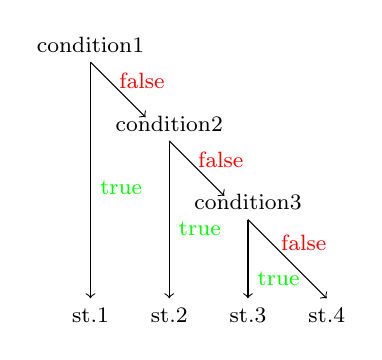
\begin{tikzpicture}[font=\footnotesize]
			\node at (0,0)[above]{condition1};
			\draw[->] (0,0) -- (0,-3) node[green, above=4em, right]{true};
			\node at (0,-3)[below]{st.1};
			\draw[->] (0,0) -- (.7,-.7) node[red, above=1.3em, right=-1.3em]{false};
			
			\node at (1,-1)[above]{condition2};
			\draw[->] (1,-1) -- (1,-3) node[green, above=2.5em, right]{true};
			\node at (1,-3)[below]{st.2};
			\draw[->] (1,-1) -- (1.7,-1.7) node[red, above=1.3em, right=-1.3em]{false};
			
			\node at (2,-2)[above]{condition3};
			\draw[->] (2,-2) -- (2,-3) node[green, above=.7em, right]{true};
			\node at (2,-3)[below]{st.3};
			\draw[->] (2,-2) -- (3,-3) node[red, above=2em, right=-2em]{false};
			
			\node at (3,-3)[below]{st.4};
		\end{tikzpicture}
		\column{0.5\textwidth}
			\begin{lstlisting}[numbers=none]
if (<condition 1>)
	<statement 1>;
else if (<condition 2>)
	<statement 2>;
else if (<condition 3>)
	<statement 3>;
else
	<statement 4>;
\end{lstlisting}
	\end{columns}
\end{frame}
\begin{frame}[fragile]{switch}
	If you have to check one variable for many constant values, \textit{switch case} is your friend:
	\begin{lstlisting}[numbers=none]
switch (<variable>) {
	case <option 1>: <statement 1>; break;
	case <option 2>: <statement 2>; break;
	case <option 3>: <statement 3>; break;
	default: <statement 4>; break;
}
\end{lstlisting}
	\begin{itemize}
	\item \textit{case $<$option$>$} defines a jump label
	\item more than one statement after it possible without braces
	\item all statements until the next \textit{break;} will be executed
\end{itemize}	 
\end{frame}
\begin{frame}[fragile]{A few words on style}

	\begin{itemize}
		\item Typing \textbf{if (cond)} instead of \textbf{if(cond)} helps people to differantiate between control structures and function calls faster
		\item when starting a new block, you should type ) \{ rather than )\{
		\item don't start a new block for a single statement
		\item don't put statements and conditions on the same line
	\end{itemize}
	\begin{lstlisting}[numbers=none]
if(cond){ statement; }	/* bad style */

if (cond) {				/* looks better, still bad style */
	statement;
}

if (cond)
	statement;			/* looks way clearer */
\end{lstlisting}
\end{frame}
\begin{frame}[fragile]{More words on style}
	\begin{itemize}
		\item if you use a block anywhere in an \textbf{if ... else} structure, put all blocks of this structure in braces
	\end{itemize}
	\begin{lstlisting}[numbers=none]
if (cond)		/* bad style, inconsistent */
	statement;
else {
	statement;
	statement;
}

if (cond) {		/* way better style */
	statement;
} else {
	statement;
	statement;
}
\end{lstlisting}
	\begin{itemize}
		\item notice: the \textit{else} is on the same line as the closing if body brace
	\end{itemize}
\end{frame}
\section{Exercises}
\subsection{}
\begin{frame}{Calculator}
	\begin{itemize}
		\item Write a Program, that takes two numbers and an operator (+, -, /, *, \%) as input and prints the result.
		\item \textbf{Experts:} The program should also accept the words \textit{add, substract, multiply, divide} and \textit{remainder} as operators.
		\begin{itemize}
			\item<2-> Hint: look at the difference between the words.
			\item<3-> Hint: how many letters do you have to check?
		\end{itemize}
	\end{itemize}
\end{frame}
\begin{frame}{Feedback}
	\begin{itemize}
		\item Write a program, that asks the user to enter a character and answers whether the input is a letter, a number, or a special char.
		\begin{itemize}
			\item<2-> Hint: have a look at the ASCII code table
		\end{itemize}
		\item \textbf{Experts:} If the character is a small letter, also print the capital letter and vice versa.
		\begin{itemize}
			\item<3-> Hint: have a closer look at the ASCII code table
		\end{itemize}
	\end{itemize}
\end{frame}
\section{Loops}
\subsection{}
\begin{frame}[fragile]{Loops}
	To repeat statements until a certain condition is met, C offers 3 different loops.
	\begin{lstlisting}[numbers=none]
while (<condition>)
	<statement>;
\end{lstlisting}
	\begin{lstlisting}[numbers=none]
do
	<statement>;
while (<condition>);
\end{lstlisting}
	\begin{lstlisting}[numbers=none]
for (<initialization>; <condition>; <statement>)
	<statement>;
\end{lstlisting}
	For multiple statements again, use braces.
\end{frame}
\begin{frame}[fragile]{while}
	The execution of a loop is a continous alternation between checking if the condition is still met and executing the statement(s).
	\begin{lstlisting}
int i = 2;
while (i > 0)
	i--;
printf("done\n");
\end{lstlisting}
	\begin{enumerate}[<+(1)->]
		\item check (i $>$ 0) $\rightarrow$ \textbf{true} $\rightarrow$ go to line 3
		\item decrement i $\rightarrow$ i now is \textbf{1}, go back to line 2
		\item check (i $>$ 0) $\rightarrow$ \textbf{true} $\rightarrow$ go to line 3
		\item decrement i $\rightarrow$ i now is \textbf{0}, go back to line 2
		\item check (i $>$ 0) $\rightarrow$ \textbf{false} $\rightarrow$ go to line 4
		\item print \textbf{done}
	\end{enumerate}
\end{frame}
\begin{frame}[fragile]{Meanwhile...}
	Be careful, this
	\begin{lstlisting}[numbers=none]
while (1 > 0)
	printf("Did you miss me?\n");
\end{lstlisting}
runs till the end of all days.\\
\ \\$\infty$ loops are common mistakes, and you will experience many of them.\\
Check for conditions that are always true.
\end{frame}
\begin{frame}[fragile]{do...while}
	The difference between \textit{do...while} and \textit{while} is the order of executing the statement(s) and checking the condition.\\
	The \textit{while} loop begins with checking, while the \textit{do...while} loop begins witch executing the statement(s).
	\begin{lstlisting}[numbers=none]
int i = 3;
do
	i--;
while (i < 1);
\end{lstlisting}
	The Statement(s) in a \textit{do ... while} loop are executed at least once.
\end{frame}
\begin{frame}[fragile]{for}
	The For-Loop is comfortable for iterating. It takes three arguments.
	\begin{itemize}
		\item initialization
		\item condition
		\item iteration statement
	\end{itemize}
	To understand how it's working, consider a program printing the numbers 1 to 10:
	\begin{lstlisting}[numbers=none]
int i;
for (i = 1; i <= 10; i++)
	printf("%d\n", i);
\end{lstlisting}
	\begin{itemize}
		\item i is called an \textit{index} whit iterates from the given start to a given end value
		\item i, j, k are commonly used identifiers for the index
	\end{itemize}
\end{frame}
\begin{frame}[fragile]{Saving code lines}
	You can define variables inside the initialization part of a for loop.
	\begin{lstlisting}[numbers=none]
for (int i = 1; i <= 10; i++)
	printf("%d\n", i);
\end{lstlisting}
	\ \\\ \\In that case, the variable is only available inside the for loop (as if it was declared in the body).\\
	But you have to compile the program with \textit{-std=c99}
	\begin{lstlisting}[numbers=none]
gcc main.c -Wall -std=c99
\end{lstlisting}
\end{frame}
\begin{frame}[fragile]{forever}
	The arguments for the \textit{for loop} are optional. E.g. if you already have defined your iterating variable:
	\begin{lstlisting}[numbers=none]
int i = 1;
for (; i <= 10; i++)
	printf("%d\n", i);
\end{lstlisting}
	Or if you have the iteration statement in your loop body:
	\begin{lstlisting}[numbers=none]
for (int i = 1; i <= 10;)
	printf("%d\n", i++);	/* why not using while? */
\end{lstlisting}
	And if you're not passing anything, it runs \textbf{for}ever:
	\begin{lstlisting}[numbers=none]
for (;;)
	printf("I'm still here\n");
\end{lstlisting}
Note: the semicolons are still there.
\end{frame}
\begin{frame}[fragile]{A few words on style}
	\begin{itemize}
		\item again, only use braces when there's more than one statement
		\item if you skip the loop body
		\begin{itemize}
			\item leave a comment in your code
			\item use an extra line for the empty statement
		\end{itemize}
	\end{itemize}
		\begin{lstlisting}[numbers=none]
for (i = 1; i < 9; printf("%d\n", i++));	/* confusing */

for (i = 1; i < 9; printf("%d\n", i++))		/* clear */
	;	/* do nothing */
\end{lstlisting}
\end{frame}
\section{More Exercises}
\subsection{}
\begin{frame}{Customized Sheldon}
	\begin{itemize}
		\item Write a program, that lets the user decide how often \textit{"Knock, knock, knock - Penny?"} is printed.
		\item \textbf{Experts:} let the program additionally ask how often Sheldon knocks each time.
		\begin{itemize}
			\item Take care, that the first "Knock" starts with a Capital K
			\item<2-> Hint: you can use loops inside loops
			\item<3-> Hint: you should use a different index for the inner loop
		\end{itemize}
	\end{itemize}
\end{frame}
\begin{frame}{Power and faculty}
	\begin{itemize}
		\item Write a program that takes two numbers $a, b$ from the user and calculates $a^b$ and $b^a$
		\item \textbf{Experts:} Write a program that calculates the factorial of the user input.
		\begin{itemize}
			\item<2-> Hint: the factor changes in each step.
		\end{itemize}
	\end{itemize}
\end{frame}
\begin{frame}{The rabbit problem}
	\begin{itemize}
		\item Write a program, that prints the $n$th fibonacci number.
		\begin{itemize}
			\item a fibonacci number is the sum of its two predecessors in the fibonacci sequence
			\item the fibonacci sequence starts with 0,1,\dots
			\item<2-> Hint: One variable is not enough to store all the information you need to calculate the next fibonacci number.
		\end{itemize}
		\item \textbf{Experts:} Also calculate the sum of all fibonacci numbers $\leq n$.
	\end{itemize}
\end{frame}
% nothing to do from here on
\end{document}
